\setchapterpreamble[u]{\margintoc}
\glsresetall % reset glossary
\chapter{Optimizing modular structures}
Introduction
\todo{change $N_T$ con $N_\text{T}$ }
\todo{NO CELLS}
\section{Formulation of a modular structure optimization algorithm}
why modular, which are the advantages

define modules and subdomains

intro there are different type of approach that we could use, full scale and multiscale

intro multiscale.

numerical homogenization

intro full scale

the problem on the number of subsections needed to correctly foresee the mechanical behaviour

\subsection{Variable linking}
\begin{figure*}
    \centering
    \includegraphics{figures/05_cellular_opt/00_modules_VL_bc/modules_bc.pdf}
    \caption{Notations used for the definition of the variable linking approach used to apply the modularity constraints.}
    \label{fig:05_VL}
\end{figure*}

In this section, we take a closer look at the Variable Linking approach. This technique involves first dividing a structure into several subdomains, which are connected during the optimization process \ie subdomains that belong to the same module all share the same cross-sectional areas. The primary goal is to make the manufacturing phase simpler and more efficient, allowing to assemble big structures starting from smaller repetitive modules. With this approach, the optimization perspective shifts. Instead of focusing on the whole structure, the optimizer design space is now restricted to the optimization of the topology of the modules.

We use \figref{fig:05_VL} to illustrate the notation employed in this thesis for modular structures. On the left-hand side of the image, we have the test case that we aim to optimize, which is already divided into $N_\text{sub}$ subdomains. Each of these subdomains is bound to exhibit the topology of one of the $N_\text{T}$ module topologies presented on the right side of the image. It is assumed that each module has the same external shape and the identical ground structure used for discretizing the module volume. Within this framework, $\bar{n}$ represents the number of candidate bars in one module, and if we assume a fully connected mesh, we can define $\bar{n}$ as $\bar{m} \cdot (\bar{m}-1)/2$, where $\bar{m}$ stands for the number of nodes in the module. Consequently, for the overall structure, we can write the relationship $N_{\text{el}} = N_{\text{sub}}\bar{n}$.

The vector that holds all the cross-sectional areas of the modules is represented as $\bar{\vect{a}}$, and it belongs to the set of positive real numbers $\mathbb{R}_+^{N_T \cdot \bar{n}}$. This vector is essentially a grouping of individual cross-sectional areas $\bar{\vect{a}}_t$ for each of the $N_T$ modules. In mathematical terms, $\bar{\vect{a}}$ is defined as follows:
\begin{equation}
    \bar{\vect{a}} :=  \{ \bar{\vect{a}}_t \in \mathbb{R}_+^{\bar{n}} \;|\; \forall t \in [1,\dots,N_T]\}
\end{equation}
The topology of the entire structure $\vect{a}$, which originates from the submodules' topology $\bar{\vect{a}}$, is defined as follows:
\begin{equation}
    \vect{a} :=  \{\vect{a}^j \;|\; \forall j \in [1,\dots,N_{\text{sub}}]\}
\end{equation}
and is evaluated using:
\begin{equation}
    \vect{a} = \sum_{t=1}^{N_T} \vect{g}_t\otimes\bar{\vect{a}}_t = \sum_{t=1}^{N_T} \begin{bmatrix}
        g_{1,t} \: \bar{\vect{a}}_t \\
        \vdots\\
        g_{N_{\text{sub}},t} \: \bar{\vect{a}}_t 
        \end{bmatrix}
\end{equation}
where the $\otimes$ operator represents the Kronecher product and $g_{t}$ represents the $t$-th column of the mapping matrix $\matr{G} = [g_0,\dots,g_{N_T}] \in \mathbb{B}^{N_{\text{sub}},N_T}$, where $\mathbb{B}=\lbrace 0,1 \rbrace$ is the Boolean domain. $g_{j,t}$ is the element at the $j$-th row and $t$-th column of the matrix $\matr{G}$. The mapping matrix $\matr{G}$ indexes are defined as follows:
\begin{equation}
    g_{j,t} =
    \begin{cases}
      1 & \text{if the $j$-th subdomain presents the topology of the $t$-th module,} \\
      0 & \text{otherwise.} 
    \end{cases}
\end{equation}
Lastly, we introduce some notation to denote specific bars within the modules and subdomains. We represent the cross-sectional area of the $i$-th bar of the $t$-th module as $\bar{\vect{a}}_{t,i}$, while the cross-sectional area of the $i$-th bar of the $j$-th subdomain as $\vect{a}^j_i$.

In the case of the structure shown in \figref{fig:05_VL} we have:
\begin{equation}
    \matr{G}=
\begin{bNiceMatrix}[first-row,last-col]
    \scriptstyle\textcolor{axis_gray}{t=0} &\scriptstyle\textcolor{axis_gray}{t=1}&  \\
    1 & 0 & \scriptstyle\textcolor{axis_gray}{\,j=0} \\
    1 & 0 & \scriptstyle\textcolor{axis_gray}{\,j=1} \\
    1 & 0 & \scriptstyle\textcolor{axis_gray}{\,j=2} \\
    1 & 0 & \scriptstyle\textcolor{axis_gray}{\,j=3} \\
    0 & 1 & \scriptstyle\textcolor{axis_gray}{\,j=4} \\
    0 & 1 & \scriptstyle\textcolor{axis_gray}{\,j=5} \\
    0 & 1 & \scriptstyle\textcolor{axis_gray}{\,j=6} \\
    0 & 1 & \scriptstyle\textcolor{axis_gray}{\,j=7} 
\end{bNiceMatrix}
\end{equation}
as the lower submodules (numbered from 0 to 3) exhibit the topology of module 0, while the upper submodules (numbered 4 to 7) represent the topology of module 1.

\subsection{Topological buckling of modular structures}
Explain only how the constraint is handled now that the cells are multiple $\bar{a}_{r}\geq \bar{a}_{r=1} \quad r \in \mathcal{C}_{l,r}(\bar{\vect{a}})$

\section{Optimization formulation}

We concentrate on the simplest type, with $N_T=1$ as there is no method to chose where to put the different modules.

the formulation $\bar{\mathbb{P}}_\text{1}$ is stated in terms of members' cross-sectional area $\bar{\vect{a}}$, member forces $\vect{q}$ and nodal displacements $\vect{U}$ as follows:
\begin{equation}
    \begin{aligned}
    \min_{\bar{\vect{a}}, \vect{q}, \vect{U}}   && V &= \vect{\ell}^{T}\vect{a}\\
    \textrm{s.t.}  && \vect{a} &= \sum_{t=1}^{N_T} \vect{g}_t\otimes\bar{\vect{a}}_t \\ 
    && \matr{B}\vect{q} &= \vect{f} && \\
    && \vect{q} &= \frac{\vect{a}E}{\vect{\ell}}\vect{b}^T\vect{U} &&  \\
    && \vect{q} &\geq -\frac{s\vect{a}^2}{\vect{\ell}^{*2}} &&  \\
    && -\sigma_c\vect{a} &\leq \vect{q} \leq \sigma_t\vect{a} &&  \\
    && \bar{a}_{r}&\geq \bar{a}_{r=1} && r \in \mathcal{C}_{l,r}(\bar{\vect{a}}) \\
    && \bar{\vect{a}} &\geq 0. \\
    \end{aligned}
    \tag{$\bar{\mathbb{P}}_\text{1}$}
    \label{eq:optim_complete}
\end{equation}

$N_{\text{sub}}$
${\bar{\vect{a}}} \in \mathbb{R}_+^{N_T \cdot \bar{n}} $ where $N_T$
${\vect{a}} :=  \{\vect{a}^j \;|\; \forall j \in [1,\dots,N_{\text{sub}}]\}$
${\bar{\vect{a}}} :=  \{ \bar{\vect{a}}_t \;|\; \forall t \in [1,\dots,N_T]\}$ represent the vector of the cross-sectional areas of the cells
$\bar{n}$ is the number of candidate bars of one cell.

Total number of design variables: $N_T\bar{n} +N_{\text{sub}}\bar{n}+2M$


number of design variables is low, buth still high constraints

\subsection{Sensitivity analysis}
how the sensitivity is changed with respect to the variable linking

just a sum more to do for constraints

\todo{image for sensitivity ?}
\section{Numerical application}
\todo{find some litterature case that we can use to compare at least visually, maybe the sandwich structure that joseph suggested me}
\subsection{On the equivalence of multi load cases and modular structures}
\begin{figure}[]
    \hspace*{\fill}
    \subcaptionbox{}{\includegraphics[height=3cm]{figures/05_cellular_opt/00_cell_multi_eq_bcs/cell_bcs.pdf}}
    \hfill
    \subcaptionbox{}{\includegraphics[height=3cm]{figures/05_cellular_opt/00_cell_multi_eq_bcs/multiload_bcs.pdf}}
    \hspace*{\fill}
    \caption{}
    \label{fig:05_cell_multi_eq_bcs}
\end{figure}

\begin{figure}[]
    \hspace*{\fill}
    \subcaptionbox{}{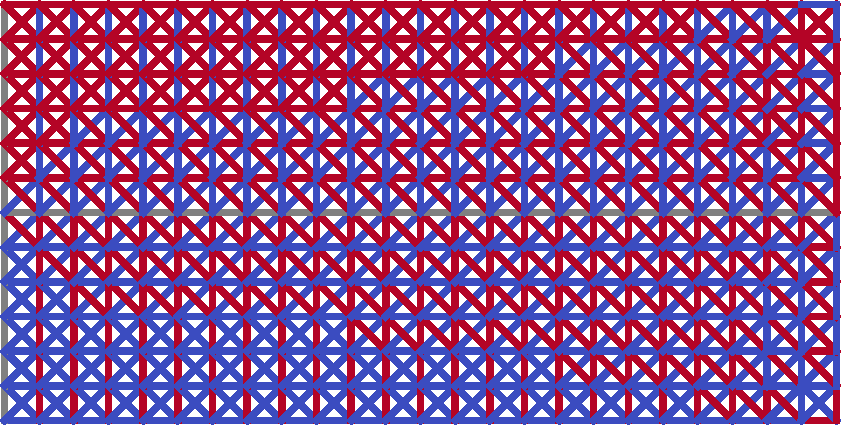
\includegraphics[height=3cm]{figures/05_cellular_opt/00_cell_multi_equivalence/cell.pdf}}
    \hfill
    \subcaptionbox{}{\includegraphics[height=3cm]{figures/05_cellular_opt/00_cell_multi_equivalence/multiload.pdf}}
    \hspace*{\fill}
    \caption{}
    \label{fig:05_cell_multi_eq}
\end{figure}
\subsection{Parametric study on the number, the shape, and the complexity of the module}

\todo{use blender to generate images}

\todo{check always the number of design variables, constraints and time}

\todo{different tables for every parametric study with iteration count}
Simply supported 3D beam

\subsection{Comparison with the optimized octet truss}


\section{Conclusion}
It's all part of our effort to strike a balance between mechanical performance and the ease of manufacturing, a topic we'll delve into further in the upcoming chapters.